%%% template.tex
%%%
%%% This LaTeX source document can be used as the basis for your technical
%%% paper or abstract. Intentionally stripped of annotation, the parameters
%%% and commands should be adjusted for your particular paper - title, 
%%% author, article DOI, etc.
%%% The accompanying ``template.annotated.tex'' provides copious annotation
%%% for the commands and parameters found in the source document. (The code
%%% is identical in ``template.tex'' and ``template.annotated.tex.'')

\documentclass[conference]{acmsiggraph}

\TOGonlineid{45678}
\TOGvolume{0}
\TOGnumber{0}
\TOGarticleDOI{1111111.2222222}
\TOGprojectURL{}
\TOGvideoURL{}
\TOGdataURL{}
\TOGcodeURL{}

\title{A Triangle Mesh Approach to Painting}

\author{Mark D. Benjamin\thanks{e-mail:mdbenjam@princeton.edu} \hspace{10 pt} Princeton Unviersity\\ Adam Finkelstein\thanks{e-mail:af@cs.princeton.edu} \hspace{10 pt} Princeton University\\ Stephen Diverdi\thanks{e-mail:diverdi@google.com} \hspace{10 pt} Google}
\pdfauthor{Mark D. Benjamin, Adam Finkelstein, Stephen Diverdi}

\keywords{triangle mesh, painting, vector graphics}

\begin{document}

%% \teaser{
%%   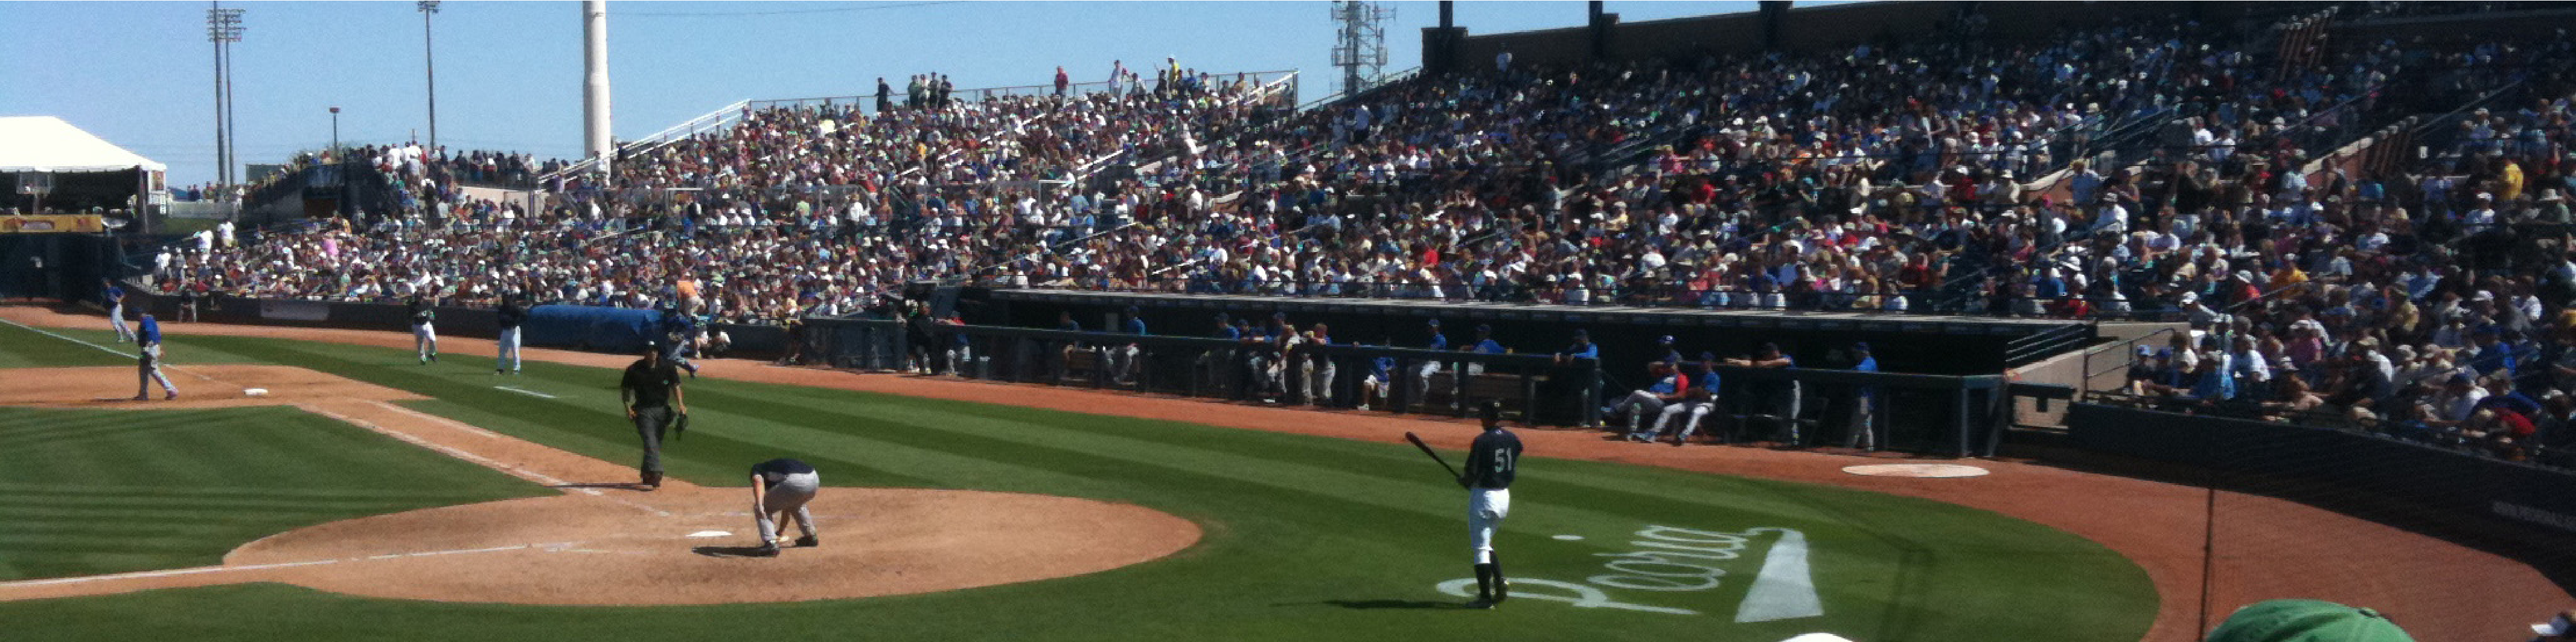
\includegraphics[height=1.5in]{images/sampleteaser}
%%   \caption{Spring Training 2009, Peoria, AZ.}
%% }

\maketitle

\begin{abstract}



\end{abstract}

\begin{CRcatlist}
  %\CRcat{I.3.3}{Computer Graphics}{Three-Dimensional Graphics and Realism}{Display Algorithms}
  %\CRcat{I.3.7}{Computer Graphics}{Three-Dimensional Graphics and Realism}{Radiosity};
\end{CRcatlist}

\keywordlist

%% Use this only if you're preparing a technical paper to be published in the 
%% ACM 'Transactions on Graphics' journal.

\TOGlinkslist

%% Required for all content. 

\copyrightspace

\section{Introduction}

All computer painting programs must store data through rasterization or vectorization. 
However, traditional computer painting programs take inputs of the same type as the stored data. The 
extremely popular Adobe programs Photoshop and Illustrator exemplify this. The former
allows a user to paint how he would on a physical medium. By letting the mouse act as
a brush, a user may color individual pixels on the screen. The latter lets a user paint
using geometric primitives such as lines and B\'{e}zier curves. The program then stores
these geometric primitives in order to render the drawing. Although using vector graphics
is likely less intuitive, it has some distinct advantages. First, there is no resolution
limit. One can zoom into an image as much as he would like and still see crisp edges.
Second, certain editing operations may be easier to perform on vector graphics.

In this paper we introduce TrianglePainter which  
uses a slightly different representation than traditional raster or vector graphics.
We instead use triangle meshes to store the data of the painting.
Since triangles are a geometric primitive used in vector graphics our approach achieves the
same advantages traditional vector graphics have. However, our representation allows the
user to paint with vector graphics without worrying about the underlying implementation.

In order to paint in our program the user simply drags his mouse on the screen to make
strokes akin to the process in a raster graphics program. Upon mouse-up the stroke is
converted to our underlying triangle mesh representation. In this way a user may paint using
vector graphics without worrying about their representation.

Furthermore, our representation allows painting at any scale. A user can make large strokes
while zoomed out and then zoom in to make fine details. All of this can happen without
loss of quality since the data is stored using triangles, not in pixels.

To do the transformation we use a combination of rasterization and marching squares to
determine the contour of the stroke. From the contour we can create a Delaunay triangulation
to represent the stroke. By then introducing a merging process we can take the triangulation
of the new stroke and combine it with the triangulation of the existing canvas. This yields
a new canvas with all the strokes combined.

TrianglePainter reduces the barriers in creating vector graphics. This in turn allows 
artists to focus on the painting and not the way in which they paint, while still 
getting the editing benefits of vector graphics.

\section{Triangulating Strokes}

Here we consider how to convert a user's cursor motion into a triangle-mesh representation
of their stroke.

\subsection{Converting Strokes to Contours}
The contour(s) define the outline of the stroke. Simply connected strokes, those without holes, have only 
one outer contour, whereas strokes with holes, such as a circle or 
figure-eight, will have more than one.
Converting a user's mouse motion into a contour requires two steps.
First, the user's mouse motion is captured by a set of polygons which can be
rendered to yield a rasterized version of the stroke.
Second, to extract the contours the stroke is rasterized in black and marching squares
is run to extract iso-contours of 50\% gray. This returns a very dense set of points 
which we reduce through a pruning process to
get a sparse but accurate representation of the contour.

\\

What do you think about this?

Note that despite the reliance on rasterization it is still possible by using
anti-aliasing and certain brushes to get sub-pixel resolution.

\subsection{Converting Contours to Triangles}
The contour contains two important pieces of information. First, it describes all of the points of the stroke.
Second, it describes the boundaries of the stroke. A triangle mesh must contain all the points and stay
within the boundaries. For example, a concave contour should not contain triangles inside the concavity.
Furthermore, these boundaries will be crucial when compositing a stroke onto a canvas.

We utilized Jonathan Shewchuk's Triangle library to perform Delaunay triangulations
on the given set of points and boundaries. The library outputs a triangle mesh that
approximately represents the drawn stroke.

\subsection{Feathered Strokes}
Finally, we must note a few changes to the above procedure in the case of feathered strokes.
Feathered strokes have two pieces, a normal inner stroke, and a ring around this stroke
where the color varies from that defined on the inner stroke to completely transparent. We
represent these strokes with two sets of points and boundaries. One set which defines the
normal inner stroke, and one set that defines the outside transparent edge of the stroke.

In order to obtain this information we must change the way we capture strokes. We accomplish
this by drawing two sets of parallelograms. One for the inner stroke and one for the outer.
When we rasterize the strokes, we do the outer one first with a color of 50\% gray and
then do the inner one second with a color of black. We run marching squares to find the
iso-contours of 25\% gray and 75\% gray and then use these two iso-contours to inform the
two sets of points and edges representing the stroke. At this point we can triangulate
the stroke normally. By providing the constraint edges and points the Triangle library will
ensure that the triangles of the outer and inner strokes do not cross the boundaries specified.

\section{Compositing Strokes}
Once the stroke has been converted to triangles by the above procedure it is necessary to
composite the stroke onto the canvas. Before drawing, every canvas is triangulated
into two large triangles. Compositing a stroke requires combining the points and boundaries
from the old strokes already on the canvas and the points and boundaries from the new stroke.
Before we get to the actual compositing, we need to understand how the triangles are colored.

\subsection{How Colors are Stored}
As we will subsequently see, the triangles on the canvas are not persistent, but the
points and boundaries from each stroke are. Therefore, all color information must be
stored in the points. All of the boundaries specify a color boundary as well. When a
stroke is drawn, on the inside of the boundary we expect the triangles to take on the
color of the stroke. On the outside of the boundary we expect the triangles to take
on the color of whatever previous strokes were laid down. In order to keep color information
stored in the points that describes the colors of the triangles, we introduce the
notion of color arcs. 

A point's color arc is a color associated with a set of two vectors such that the point 
will take on the color for any triangle it is a part of whose centroid lies within the 
color arc. Points can have multiple color arcs. The union of all of the color arcs should
cover all $2\pi$ radians around the point. And no two color arcs should intersect.
In this way for any triangle formed with a given point, the point's color assignment within
that triangle can be uniquely determined by finding which color arc the centroid is in. 

\subsection{Finding Modified Points}
One way to create our new triangulation of the canvas is to add our points and boundaries
to the old list of points and boundaries and have Triangle perform a Delaunay triangulation
of the entire set. Since this triangulation will preserve the boundaries we provided,
(i.e. no triangles will cross any of the constraint edges) all of the strokes will be
defined by a set of triangles. There is clearly a way to color these triangles to
correctly represent the strokes. We discuss how to find the colors in subsequent sections.

However, a canvas may easily contain thousands of triangles, and a new stroke may only 
intersect some small subset of them. It seems wasteful in terms of computational
resources to perform a re-triangulation of the entire canvas when most of the triangles
are not affected by this new stroke. This also means we can't keep the effects of
strokes local. In other words a stroke in the bottom left may have an effect in the top
right.

In order to solve this problem our program selectively choses which triangles can remain
and which triangles need to be included in the re-triangulation. We make a 20-by-20 grid
and mark all of the cells which contain one a triangle from the new stroke. We then
find the set of triangles from the old triangulation that intersect these grid squares.
The set of edges from these triangles that do not intersect these grid cells form a ring
around the area of our new triangles. We make all of the edges in this ring into constraints
in our triangulation. All of the points and constraint edges from the old triangulation are
included as well as the points and constraint edges from the new triangulation. Triangulating
these points and edges gives the new geometry for the area we're concerned with, but due
to the ringed constraint edges it has no effect on any other part of the canvas. Therefore
we can reuse the old triangles from the rest of the canvas. Together the new triangulation
plus the old triangle gives a new triangle mesh representation of the entire canvas.

\subsection{Determining Colors}
The final piece of the algorithm is to determine the color arcs for each of the points.
When first putting down points from a stroke, color arcs are immediately assigned. For
a normal stroke there are two color arcs. The first arc has the color of the current
brush and covers the inside of the stroke. The second arc has the color of whatever color was
already there before this point and covers the outside of the stroke. To determine
what color was already there we do a point in triangle test on the current canvas. This
gives us the triangle, and since we know the color arcs of the three vertices, we can calculate
with bilinear interpolation the color at the concerned point.

For a feathered stroke points only have one color arc. For the inner stroke the color arcs
go all $2\pi$ radians around and have the color of the stroke. For the outer stroke the
color arcs go all $2\pi$ radians around and are whatever color was there before. This means
that all triangles between the inner and outer strokes will have a linear change in color
from this stroke's color, to that of the surrounding.

Whenever a new stroke is composited on an old stroke there will be a change in the color of
any point that is now covered. The vectors defining the arc remain the same, but the color
itself will be the new color of the stroke over the old color of the arc. In the case of a
feathered stroke, where some parts of the stroke have changing color, the color of that
triangle at that point must be calculated by bilinear interpolation.

Finally, the most interesting case is when constraint edges intersect. When performing the 
triangulation of the new stroke on top of the old strokes, in most situations constraint
edges will intersect. Since no triangle can pass through these edges it is necessary for a point
to be added at the intersection. The Triangle library does this automatically. However, this
intersection point has no color data since we did not create it when we created the
stroke.

To determine the color data for an intersection point it is necessary to follow the constraint
edges to find points with color data. Note that the neighboring points may be intersection
points as well and therefore not have any color data. Once we've found colored points we
linearly interpolate the color arcs from either side of our intersection point to determine 
the colors at our new point. Once we have the average color arcs from both directions we
composite the color arcs of the new stroke over that of the old stroke in order to get four
color arcs of the four combinations of the old color arcs.

\subsection{Discussion}
Our work with this algorithm has lead to observations in three main areas.

\subsubsection{Stability}
Something we've worked hard to achieve is program stability. Certain geometries are fatal
for the Triangle library. The current instability in the program is normally caused by
providing the library with such difficult geometries. To improve program stability would
require addressing geometries such as vertices that are too close together. This would
take more processing time and is something we have yet to explore. However, clearly this
problem must be solved before the program could be used formally.

\subsubsection{Performance}
The current implementation uses Python and PyOpenGL. Python's performance is worse than
a lower level implementation in C++ would be. The drawing of the canvas is quick with
no lag. However, the actual process to extract a stroke from rasterization to triangle
representation on the canvas is slow. On a blank canvas strokes take on the order of
1 second to process. However, on a canvas with lots of geometry a stroke that covers
that geometry can take several seconds to render. Some of this time is due to poor
implementation of the algorithm. However, there are lots of calculations
to do with the old points affected by the new stroke and the points associated with the
new stroke itself. Since these geometries can get arbitrarily complicated, these
calculations can take an arbitrarily long. This brings us to the final point, scalability.

\subsubsection{Scalability}
No matter how good the implementation, the fact that paintings can get arbitrarily complicated
means there must be some way to simplify the mesh. Although we have yet to implement
such a simplification algorithm, we have discussed the possibility. In most situations where
a lot of strokes are composited on top of one another, most of the geometry is redundant. 
For example, when an opaque stroke is laid down on top of a complex geometry, that complex
geometry no longer has any useful information since the outline of the opaque stroke
completely defines it. Furthermore, even with translucent or feathered strokes, enough
composited strokes may produce complex geometry that does not add much to the output.
Some of this geometry can be reduced without noticeable changes in the output. Such a
simplification algorithm must be implemented to ensure a painter can continue to paint
without the program slowing to an unusable state.

\section{Results}

\section{Conclusion}

\section*{Acknowledgements}

\bibliographystyle{acmsiggraph}
\bibliography{template}
\end{document}
